%\iffalse
\let\negmedspace\undefined
\let\negthickspace\undefined
\documentclass[journal,12pt,twocolumn]{IEEEtran}
\usepackage{cite}
\usepackage{amsmath,amssymb,amsfonts,amsthm}
\usepackage{algorithmic}
\usepackage{graphicx}
\usepackage{textcomp}
\usepackage{xcolor}
\usepackage{txfonts}
\usepackage{listings}
\usepackage{enumitem}
\usepackage{mathtools}
\usepackage{gensymb}
\usepackage{comment}
\usepackage[breaklinks=true]{hyperref}
\usepackage{tkz-euclide} 
\usepackage{listings}
\usepackage{gvv}                                        
\def\inputGnumericTable{}                                 
\usepackage[latin1]{inputenc}                                
\usepackage{color}                                            
\usepackage{array}                                            
\usepackage{longtable}                                       
\usepackage{calc}                                             
\usepackage{multirow}                                         
\usepackage{hhline}                                           
\usepackage{ifthen}                                           
\usepackage{lscape}

\newtheorem{theorem}{Theorem}[section]
\newtheorem{problem}{Problem}
\newtheorem{proposition}{Proposition}[section]
\newtheorem{lemma}{Lemma}[section]
\newtheorem{corollary}[theorem]{Corollary}
\newtheorem{example}{Example}[section]
\newtheorem{definition}[problem]{Definition}
\newcommand{\BEQA}{\begin{eqnarray}}
\newcommand{\EEQA}{\end{eqnarray}}
\newcommand{\define}{\stackrel{\triangle}{=}}
\theoremstyle{remark}
\newtheorem{rem}{Remark}
\begin{document}
\bibliographystyle{IEEEtran}
\vspace{3cm}
\title{\textbf{11.9.3.7}}
\author{EE23BTECH11210-Dhyana Teja Machineni$^{*}$% <-this % stops a space
}
\maketitle
\newpage
\bigskip

\textbf{QUESTION:}\\
Find the sum to indicated number of terms in each of the geometric progressions in
0.15, 0.015, 0.0015, ... 20 terms.
\section*{Solution}
 
\begin{flushleft}
     \begin{table}[h]
         \caption{Variables and their descriptions}
         \label{tab:table2}
         \renewcommand{\arraystretch}{1.5}
\begin{tabular}{|c|c|c|}
\hline
Parameter & Description & Value \\\hline
\( n \) & No. of terms in the G.P &20 \\\hline
\(x(0) \) & first term in the G.P&0.15 \\\hline
\( r \) & common ratio in the G.P& 0.1 \\\hline
\( x(n) \) & nth term in the G.P& none \\\hline
\( X(z) \) & Z transform of x(n)& none \\\hline
\( Y(z) \) & Z transform of y(n)& none \\\hline
\(y(n)\)& Sum of n terms of GP& none\\\hline
\end{tabular}

     \end{table}
 \end{flushleft}
\begin{align}
x(n) &= x(0)r^n \\
X(z)&= \sum_{n=-\infty}^{\infty}x(0) r^n u(n) z^{-n}\\
X(z)&= \sum_{n=0}^{\infty}x(0) r^n z^{-n}\\
X(z) &= \frac{x(0)}{1-rz^{-1}} \qquad |z| > |r| \\
U(z)&=\frac{1}{1-z^{-1}}, \qquad |z|>1\\
S(z)&=\sum_{n=-\infty}^{\infty}s(n) z^{-n}\\
s(n)&= x(n)*u(n)\\
S(z)&=X(z)U(z)\\
&= \left( \frac{x(0)}{1-rz^{-1}}\right)\left(\frac{1}{1-z^{-1}} \right),\qquad |z| > 1  \qquad |z|>|r|
\end{align}
Use Counter integration to find the inverse of the z transform which gives sum of n terms
\begin{align}
s(n)&= \frac{1}{2\pi j}\oint_C S\brak{z}z^{n-1}dz\\
&=\frac{1}{2\pi j}\oint_C \frac{x(0) z^2}{(z-1)(z-r)}z^{n-1} dz\\
&= \frac{1}{\brak{m-1}!}\lim_{z\to\ a}\frac{d^{m-1}}{dz^{m-1}}\brak{\brak{z-a}^m f\brak{z}}\\
 &= \lim_{z\to \ 1}\frac{d}{dz}\brak{\brak{z-1}^2 \frac{x(0) z^{n+1}}{(z-1)(z-r)}}\\
 &=\lim_{z\to \ 1}\frac{d}{dz}\brak{\brak{z-1} \frac{x(0) z^{n+1}}{(z-r)}}
\end{align}
\hspace{0.5cm}    solving equation(13) we get sum of n terms of the given GP
\begin{align}
    s(n)&= \frac{x(0)}{1-r}\\
    &=\frac{0.15}{0.9}\\
    &=0.16667
\end{align}
        $\therefore$ Sum of 20 terms of the given GP is $0.16667$
       \renewcommand{\thefigure}{\theenumi}
 \renewcommand{\thetable}{\theenumi}
 
\begin{figure}[h]
  \centering
  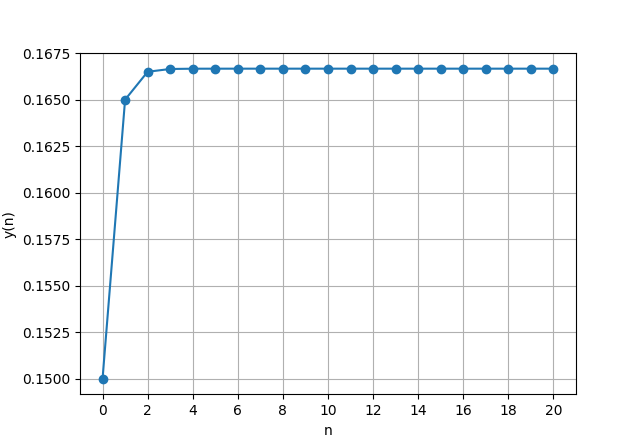
\includegraphics[width=0.6\textwidth]{figs/graph.png}
  \caption{SUM OF n TERMS OF GP}
  \label{fig:your_label}
\end{figure}


\end{document}
